\documentclass[12pt,a4paper]{article}

\usepackage{fontspec}
\usepackage{polyglossia}
\usepackage[left=3cm,top=2cm,right=1cm,bottom=2cm,nohead]{geometry}
\usepackage{setspace}
\usepackage{listings}
\usepackage{graphicx}
\usepackage{color}
\usepackage{float}
\usepackage{caption}
\usepackage{subcaption}
\usepackage{courier}
\usepackage{bold-extra}
\usepackage{fix-cm}
\usepackage{alltt}
\usepackage{indentfirst}
\usepackage{amsmath, amsthm, amssymb}
\usepackage{url}

\defaultfontfeatures{Mapping=tex-text}

\setmainfont
    [ Path           = fonts/ ,
      UprightFont    = *-Regular,
      BoldFont       = *-Bold ,
      ItalicFont     = *-Italic ,
      BoldItalicFont = *-BoldItalic]
    {LiberationSerif}
\setsansfont
    [ Path           = fonts/ ,
      UprightFont    = *-Regular,
      BoldFont       = *-Bold ,
      ItalicFont     = *-Italic ,
      BoldItalicFont = *-BoldItalic]
    {LiberationSans}
\setmonofont
    [ Path           = fonts/ ,
      UprightFont    = *-Regular,
      BoldFont       = *-Bold ,
      ItalicFont     = *-Italic ,
      BoldItalicFont = *-BoldItalic]
    {LiberationMono}

\setmainlanguage{ukrainian}
\setotherlanguage{english}



\graphicspath{{./images/}}

\setstretch{1.1}

\definecolor{javared}{rgb}{0.6,0,0}
\lstdefinelanguage{Smalltalk}{ 
  morekeywords={true,false,self,super,nil}, 
  sensitive=true, 
  morecomment=[s]{"}{"}, 
  morestring=[d]', 
} 
 
\lstset{
	basicstyle=\footnotesize\ttfamily,
	tabsize=3,
	showspaces=false,
	stringstyle=\color{javared},
	showstringspaces=false,
	xleftmargin=	.6cm
}

\begin{document}
\pretolerance=-1
\tolerance=2300

\pagenumbering{arabic}
\pagestyle{empty}
\setlength{\parindent}{1.5cm}
\fontsize{14pt}{6mm}\selectfont

\begin{center}
  \begin{spacing}{2}
    \uppercase{
      Львівський національний університет імені Івана Франка
      
      Факультет прикладної математики та інформатики 
       
      Кафедра програмування
    }
  \end{spacing}

  \vspace{6cm}


    {\bfseries\Large Магістерська робота}

    {\small (освітньо--кваліфікаційний рівень магістр)}
    
    \bigskip   
    
    на тему: {\bfseries\large „Розширення функціональності моделі FAMIX для побудови абстрактних дерев коду Java-- та Smalltalk--програм“}

\end{center}

\vspace{2cm}

\begin{small}
\begin{flushleft}\leftskip8.5cm
  Виконав студент 5 курсу, групи ПМІ-51м спеціальності 8.04030201 Інформатика\\
  Тимчук Ю.А.\linebreak
  
  Керівник: доц. Рикалюк Р.Є.\linebreak
  
  Рецензент:   
  
\end{flushleft}
\end{small}

\vspace{5cm}

\begin{center}
  Львів - 2013 року
\end{center}

\clearpage



\setstretch{1.5}
\fontsize{14pt}{6mm}\selectfont

\tableofcontents
\clearpage
\pagestyle{plain}
\section{Вступ}

Метамоделювання було створено для того, щоб дозволити розглядати програми на вищому рівні абстракції, ніж це забезпечують звичайні мови програмування. Основна ідея такого програмування полягає в тому, що розробник визначає високорівневу модель рішення, описує, як перетворити це рішення в програму для певної мови, а потім автоматично генерує вихідний код програми. В ідеалі такий же підхід дозволяє взяти існуючу програму, автоматично побудувати її абстрактну модель, вручну розширити або поліпшити модель і згенерувати нову програму, можливо, новою мовою програмування (round-trip engineering). Такий підхід був би дуже цікавим для організацій, що мають програми, написані із застосуванням старих технологій (наприклад, мови Cobol) і хочуть перенести їх на більш сучасні платформи (наприклад, Java, Ruby, тощо). Науково--дослідницька команда RMoD національного францьзького інституту INRIA вже має інструменти, які можуть приймати програми написані мовами C, Java, Smalltalk в якості вхідних даних і продукувати з них моделі.

Проте завдання генерувати програму за її моделлю висуває суперечливі вимоги до цієї моделі: вона мала б бути досить детальною щоб дати змогу відновити повний текст програми. Ця потреба, звичайно, не сумісна з ідеєю абстрагування моделі програми. Тому потрібно бути в змозі створити абстрактну модель програми, але, в той же час, створити дуже детальну модель тієї ж програми і таким чином, мати можливість працювати на двох рівнях абстракції одночасно.

Як приклад можна розглянути дві об'єктно-орієнтовані мови програмування: Java та Smalltalk. Обидві мають подібну структуру: класи, поля та методи класів. Але у мові Smalltalk відсутні інструкції галуження та циклу, які, безперечно, відіграють важливу роль в Java коді. З другого боку, код Java не має нічого аналогічного до блоків у мові Smalltalk, які дозволяють реалізовувати галуження та цикли за допомогою методів.

На даний момент для моделювання вихідного коду на високому рівні використовується метамодель FAMIX, яка надає змогу моделювати пакети, класи, методи, змінні та взаємозв'язки між цими сутностями. Метою цієї магістерської роботи є розширення метамоделі FAMIX шляхом додавання до неї компонент абстрактних синтаксичних дерев мов програмування Java та Smalltalk.

\subsection{Перспективи використання}
Абстрактні синтаксичні дерева зазвичай використовуються при компіляції, коли для нас важлива лише функціональна складова даних, маючи яку ми зможемо згенерувати байтко програми, який буде виконуваті дії записані у вихідному коді. Основне завдання даної моделі --- збереження інформації у такій структурі, яка дозволить легко аналізувати вихідний код, а також генерувати його. Це передбачає збереження якомога більшої кількості інформації у моделі.

Маючи в своєму розпорядженні універсальне дерево, яке можна буде розширювати для різних мов, дотримуючись простх правил, можна розробляти алгоритми, які будуть працювати для всіх розширень дерева. Таким чином, можна буде зробити інструмент для моделювання програм, написаних, практично, будь--якою мовою програмування без значних затрат ресурсів. Серед можливих завдань можна виділити:

\textbf{Розпізнавання символів}: сутність змінної в абстрактних синтаксичних деревах несе лише інформацію про назву змінної, цього доволі мало для аналізу вихідного коду. Однаковий ідентифікатор може зустрічатись в різних місцях програми, але стосуватися різних змінних.

\textbf{Інтерфейс взаємодії}: модель --- це лише пов'язані між собою сутності з параметрами. Для полегшення роботи з моделлю потрібно розробити первинний інтерфейс взаємодії, наприклад: графічну оболонку, мову запитівб тощо.

\textbf{Перевірка правил}: маючи модель вихідного коду можна реалізувати перевірку деяких правил, щоб виявити „поганий“ код, як, наприклад, \lstinline$if (false) {...}$.

\textbf{Генерація коду з моделі}: якщо можна було б генерувати код програми з наявної моделі, то це б можна було використати для рефакторингу програм шляхом взаємодії з графом моделі у графічному інтерфейсі. Можливо аналогічний підхід можна було б застосовувати для побудови програм.

\textbf{Перетворення між мовами}: маючи в наявності реалізацію вищезазначеного функціоналу можна було б розробити перетворення коду з однієї мови в іншу. Звичайно, неможливо написати алгоритм, який буде генерувати ідеальний код новою мовою програмування, але навіть можливість згрубша перевести програмне забезпечення, яке складається з мільйонів рядків коду було б корисною можливістю.

\subsection{Постановка задачі}
На початку виконання роботи з уже наявного матеріалу можна виділити метамодель FAMIX та платформу для аналізу даних Moose. 

Головною метою задачі є створення загальної метамоделі абстрактного синтаксичного дерева, яке з легкістю можна розширювати для моделювання тої чи іншої мови. В результаті повинна бути створена певна базова модель, а також правила та приклади її розширення.

Першочерговою ціллю є створення повноцінної метамоделі для моделювання програм написаних мовою програмування Smalltalk. Таким чином буде можливість перевірити правильність моделі для конкретної мови програмування. Причина вибуру мови Smalltalk для реалізації першої повної моделі --- простота мови, яка дозволяє за короткий час змодельвати усі конструкції цієї мови програмування.

Після повноцінної реалізації моделі для мови програмування Smalltalk, наступною ціллю є реалізація декількох простих алгоритмів з метою перевірки практичності моделі, а також аналізу важливості тих чи інших властивостей моделі.

Після виконання попередніх досліджень заключним етапом є розширення метамоделі для моделювання коду написаного мовою програмування Java. Причина вибуру мови Java для реалізації другої моделі полягає в тому, що Java --- одна з найбільш вживаних мов програмування і дуже відрізняється від мови програмування Smalltalk, для якої було сторено перше розшинення метамоделі. На цьому етапі важливим є першочергове моделювання окремих ланок мови, які дозволяють показати вірність метамоделі, а також перевірку коректності алгоритмів та задач реалізованих на попередньому кроці. Для створення повноцінної метамоделі мови програмування Java може знадовитися дуже велика кількість часу, що зумовлено складністю мови, тому це не є основною задачею.

В кінці виконання завдання метамодель має бути сумісною з моделлю FAMIX, та підтримувати основні властивості платформи Moose. 

\clearpage

\section{Moose}

В рамках цієї роботи використовується платформа з відкритим кодом Moose\cite{moose}, яка призначена для аналізу систем програмного забезпечення та даних в цілому. Ця платформа написана на мові програмування Smalltalk та інтегрується безпосередньо в середовище Pharo. Ядро Moose надає можливість збереження та взаємодії із сутностями моделей. Для цього використовуються три базові класи: \emph{Entity}, \emph{Group} та \emph{Model}.

Клас Entity(сутність) є базовим представленням сутності у моделі. Тому передбачено, що конкретні сутності специфічних метамоделей будуть наслідуватись саме від цього класу. Entity надає два загальні сервіси. Перший - це зв'язок з моделлю до якої належить дана сутність. Це веде до циклічної залежності між моделлю та сутністю, але з одного боку така реалізація нікому не заважає, а з другого - дозволяє легко формувати запити, які потребують більшу кількість інформації аніж дана сутність може надати. Другою важливою особливістю Entity є механізм управління станами і розширенням, який досягається за рахунок ієрархії EntityState. Ця ієрархія надає словник, в якому можна зберігати дані про сутність, зокрема кешувати дані отримані під час виконання запитів.

Клас Group(група) - це сутність, яка відображає колекцію сутностей. Наприклад, у нас може бути група сутностей класів, чи група сутностей методів. Групи є важливою абстракцією, особливо для виконання запитів та користувацького інтерфейсу.

Клас Model(модель) по своїй суті є сукупністю сутностей та їх внутрішніх зв'язків для вибраної системи. Це спеціальний підвид групи.

Moose використовує сім'ю мета-моделей під назвою FAMIX. Вони можуть бути використані для представлення моделей пов'язаних з різними аспектами систем програмного забезпечення. Ці мета-моделі зазвичай спрямовані на полегшення аналізу,  і надають багатий API для здійснення запитів та навігації. Ядро FAMIX складається з узагальненої мета-моделі, яка може відобразити багато об'єктно--орієнтованих та процедурних мов. 

\clearpage

\section{Основні ідеї FAST}

FAST являє собою інфраструктуру з трьох частин: модель, завантажувач та додатки.

Основна ідея \emph{моделі} --- це визначення структури, яку можна буде використовувати для репрезентації коду у вигляді абстрактного синтаксичного дерева. Ця модель слідує основним принципам FAMIX. Тобто створюється ядро моделі, яке визначає структуру однакову для всіх мов програмування. Тоді для кожної мови програмування створюється розширення, яке додає свої специфічні ланки.

Щоб ця система була актуальною для використання, необхідно мати можливість генерувати моделі безпосередньо з вихідного коду методу. Для цього використовується \emph{завантажувач}. Він слідує попередній стратегії, втім ядро завантажувача доволі мале, так як кожна мова вимагає окремого підходу для завантаження.

\emph{Додатки} мають на меті опрацювання моделі. Тобто алгоритми для визначення метрик, або відвідувач для траверсу моделі. Основна ідея додатків полягає в тому, що вони не мають сильно відрізнятись для кожної мови (крім відвідувача).

\subsection{Модель}

Абстрактне синтаксичне дерево зазвичай використовується компілятором як основа для генерування байт--коду. В нашому ж випадку модель абстрактного синтаксично дерева має містити якомога більше кількість інформації для того, щоб дозволити нам проводити аналіз різного типу на її основі. З цією ж метою метамодель, яку ми розробляємо буде максимально зв'язаною з існуючою метамоделлю.

\textbf{Вираз (Expression)} --- це частина коду, яка має певне значення. Це може бути літерал, змінна, виклик функції (чи методу). Вираз може бути присвоєним змінній чи переданим як аргумент.

Виконавче тіло методу складається з \textbf{речень (Statement)}. Кожне речення являє собою повноцінну виконавчу ланку. Яскравими прикладами речень є інструкція галуження \lstinline$if$, інструкції циклів, або ж речення, яке вказує на повернення з методу. Також часто зустрічаються речення які просто містять вираз, наприклад:
\begin{lstlisting}[language=Java]
System.out.printl("Hello world");
\end{lstlisting}

Часто важко побачити різницю між виразами та реченнями. Перш за все збивають речення які не містять нічого іншого крім виразу. Наприклад
\begin{lstlisting}[language=Smalltalk]
5 factorial
\end{lstlisting}
це вираз. Ми його можемо передати як параметр повідомлення або ж відправити повідомлення йому самому:
\begin{lstlisting}[language=Smalltalk]
'Factorial of 5: ', 5 factorial asString
\end{lstlisting}
Наступний приклад є реченням:
\begin{lstlisting}[language=Smalltalk]
5 factorial.
\end{lstlisting}
В смолтоці крапки використовуються як розділювачі для речень. Даний приклад доволі концептуальний, але головне його покликання --- показати, що речення --- це сутності на найвищому рівні виконавчого коду. І не зважаючи на те, що деякі речення можуть складатись з лише одного виразу --- це всеодно речення і вони є абсолютно відмінними від сутностей.

З другого боку різні мови мають різні правила. Наприклад в смолтоку присвоєння є виразом, тому ми можемо написати:
\begin{lstlisting}[language=Smalltalk]
list add: x := 5 factorial
\end{lstlisting}
цей код обчислить $5!$ присвоїть його змінній $x$ а потім додасть ці значення до списку. В мові програмування \emph{Basic} присвоєння є реченням, це також часто призводить до непорозумінь між термінами.

Давайте розглянемо приклад:
\begin{lstlisting}[language=Smalltalk]
middleOf: a and: b
    | sum |
    sum := a + b.
    ^ sum / 2
\end{lstlisting}
Перші два рядки відносяться до оголошення методу та тимчасових змінних, тому зараз можемо їх опустити. У даному прикладі присутні два \emph{речення}:
\begin{enumerate}
	\item \lstinline$sum := a + b$
	\item \lstinline$^ sum / 2$
\end{enumerate}
А також близько пів--дюжини \emph{виразів}: \lstinline$sum := a + b$, \lstinline$sum$, \lstinline$a + b$, \lstinline$a$, \lstinline$b$, \lstinline$sum / 2$, \lstinline$2$.

Не зважаючи на те, що я розробляю окремі моделі для кожної з мов, за основу було вибрано ідею, яка передбачає стандартні правила для всіх моделей. Цю ідею можна сформулювати наступним чином:
\begin{enumerate}
  \item Виконавча частина функції(методу) є послідовністю речень.
  \item Речення може містити вирази або ж виконавчі блоки.
  \item Виразом є сутність, яка має значення.
\end{enumerate}
Тому в наступних моделях у нас будуть присутні базові типи \emph{речення} та \emph{вираз}, при чому без будь-яких безпосередніх зв'язків. Звичайно, в їхні наслідники можуть залежати одне від одного, але на найвищому рівні ми таких обмежень не накладаємо.

В якості узагальнення всіх посилання на сутності за допомогою їхнього ім'я використаємо \textbf{іменовану сутність (Named Entity)}. Прикладом може бути використання будь-якої змінної для присвоєння їй значення чи використання значення на яке вона вказує, або ж назва класу метод якого буде викликатись. Ця сутність буде зв'язана з іменованою сутністю FAMIX, яка в свою чергу може бути локальною чи глобальною змінною, параметром, змінною класу, неявною змінною, або ж класом.

\textbf{Сутність з поведінкою (Behavioural Entity)} - це сутність, яка має в собі певний код, який виконується --- поведінку. Наприклад методи, функції, замикання та лямбда--функції є такими сутностями. Ця сутність має набір \emph{речень}, а також два набори \emph{іменованих сутностей} в якості параметрів та локальних змінних. \emph{Сутність з поведінкою} буде слугувати коренем для нашого дерева. Логічним розширенням буде \textbf{іменована сутність з поведінкою (Named Behavioural Entity)}, так як методи та функції мають ім'я чи селектор за яким їх можна ідентифікувати. \emph{Іменована сутність з поведінкою} в свою чергу буде зв'язана з іменованою сутністю FAMIX, так як остання передбачає в собі наявність селектора.

\begin{figure}[h]
  \centering
    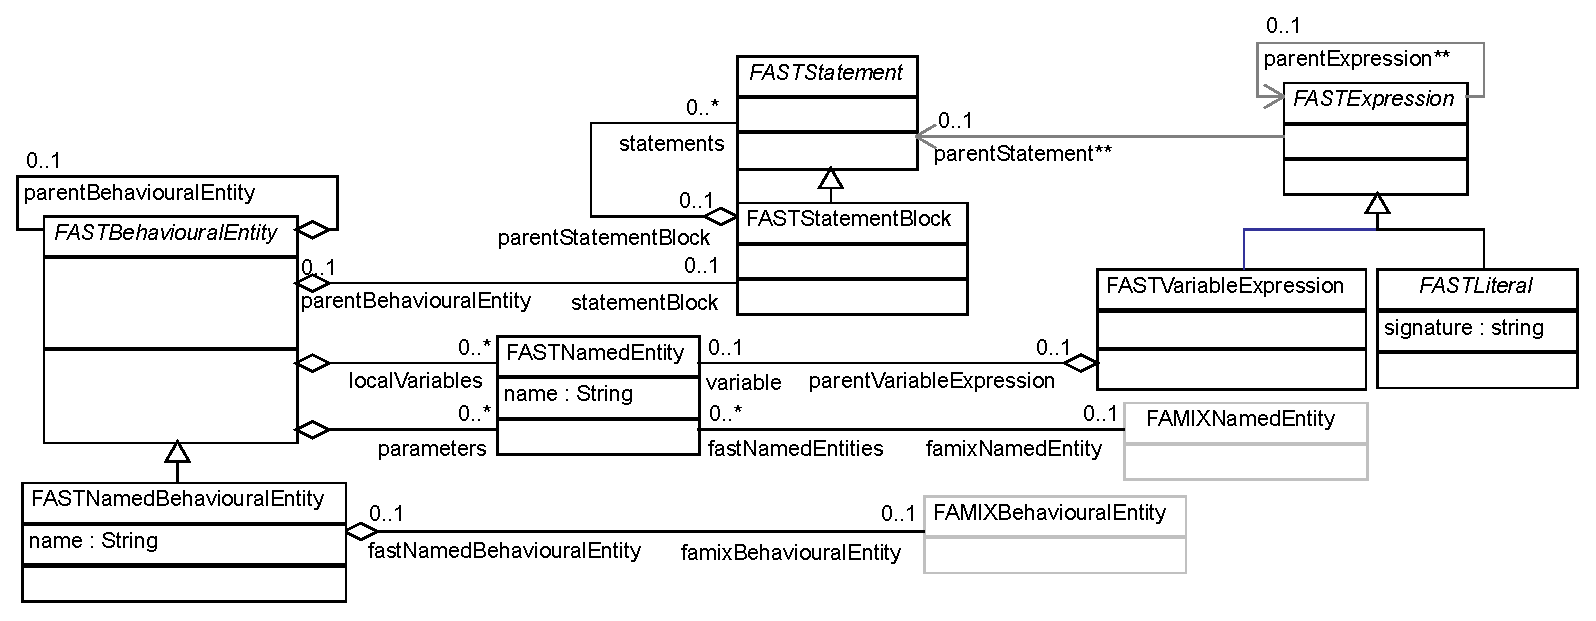
\includegraphics[width=0.95\textwidth]{GeneralASTClassDiagram}
  \caption{Базова структура FAST\label{genFast}}
\end{figure}

На рис.~\ref{genFast} показано діаграму основи моделі. Префікс \textbf{FAST} - це назва моделі, означає він Famix AST.

\subsubsection{Квазі--загальні ланки}

Посеред мов програмування присутні подібні конструкції, які можуть зустрічатись не у всіх мовах, або ж мати невелику різницю. Наприклад, це речення, яке повертає значення з методу. З одного боку --- це дуже поширена конструкція, яка просто незамінна у багатьох мовах програмування. З другого --- синтаксис у Smalltalk та Java дещо інший, ланка повернення для обох мов має себе поводити дещо інакше. Також, якщо подивитись на функціональну мову програмування SML, то в неї немає такого поняття, як речення, що повертають значення, адже кожне речення має цю поведінку. Якщо ж вважати, що кожне речення SML є ланкою повернення, то звідси випливає, що в таких мовах немає речення, яке містить просто вираз. На даний момент прийнято рішення в кожній мові визначати свої ланки. Наприклад в поточній реалізації мають місце ланки FASTSmalltalkReturnStatement та FASTJavaReturnStatement.

\subsection{Завантажувач}

Основна ідея завантажувача --- це сотворення абстрактного синтаксичного дерева за метамоделлю FAST з вихідного коду. Загальна ідея завантаження на даний момент полягає у використанні PetitParser для генерації абстрактного синтаксичного дерева, яке притаманне самій мові, з вихідного коду. Далі відвідувач траверсує це дерево, і на базі нього утворює дерево FAST. Парсер являє собою зовнішній пакет, який не належить безпосередньо до нашої системи, в той час, як відвідувач --- специфічний для кожної мови. Крім того він наслідує абстрактного відвідувача, який зазвичай є частиною пакету парсера реалізованого на PetitParser. Втім для уникнення дуплікації коду, деякі спільні методи були винесені в спільний трейт TFASTImporterVisitor. Ці методи являють собою запуск парсера для певної частини коду, та додавання елементу для до моделі.

Варто зауважити, що використання PetitParser не є примусовим. Наприклад, можливим є сценарій, коли завантажувач буде запускати зовнішню програму, передавати їй код, отримувати результат в проміжному вигляді і опрацьовувати його. Таким чином, можливо цьому завантажувачу функціонал трейту TFASTImporterVisitor буде непотрібним.

\clearpage

\section{Метамодель абстрактного дерева Smalltalk}

Абстрактне синтаксичне дерево смолтоку вражає. Не зважаючи на те, що у FAST--варіанті смолтоку присутні „зайві“ ланки, які призначені для сумісності з іншими мовами, це дерево складається лише з двадцяти семи ланок. Навіть синтаксис смолтоку містить в три рази менше граматичних елементів аніж синтаксис джава\cite{meet-grammars}. Робота з смолтоком була першою ціллю цього проекту, так як абстрактне синтаксичне дерево достатньо мале і просте, для того, щоб його змоделювати повною мірою. В той же час смолток являє собою повноцінну мову, на якій можна реалізувати рішення основних проблем, які виникають при еволюції програмного забезпечення.

\subsection{Структура моделі}

Діаграма класів моделі абстрактного синтаксичного дерева смолтоку рис.~\ref{smtFast}.

\begin{figure}[h]
  \centering
    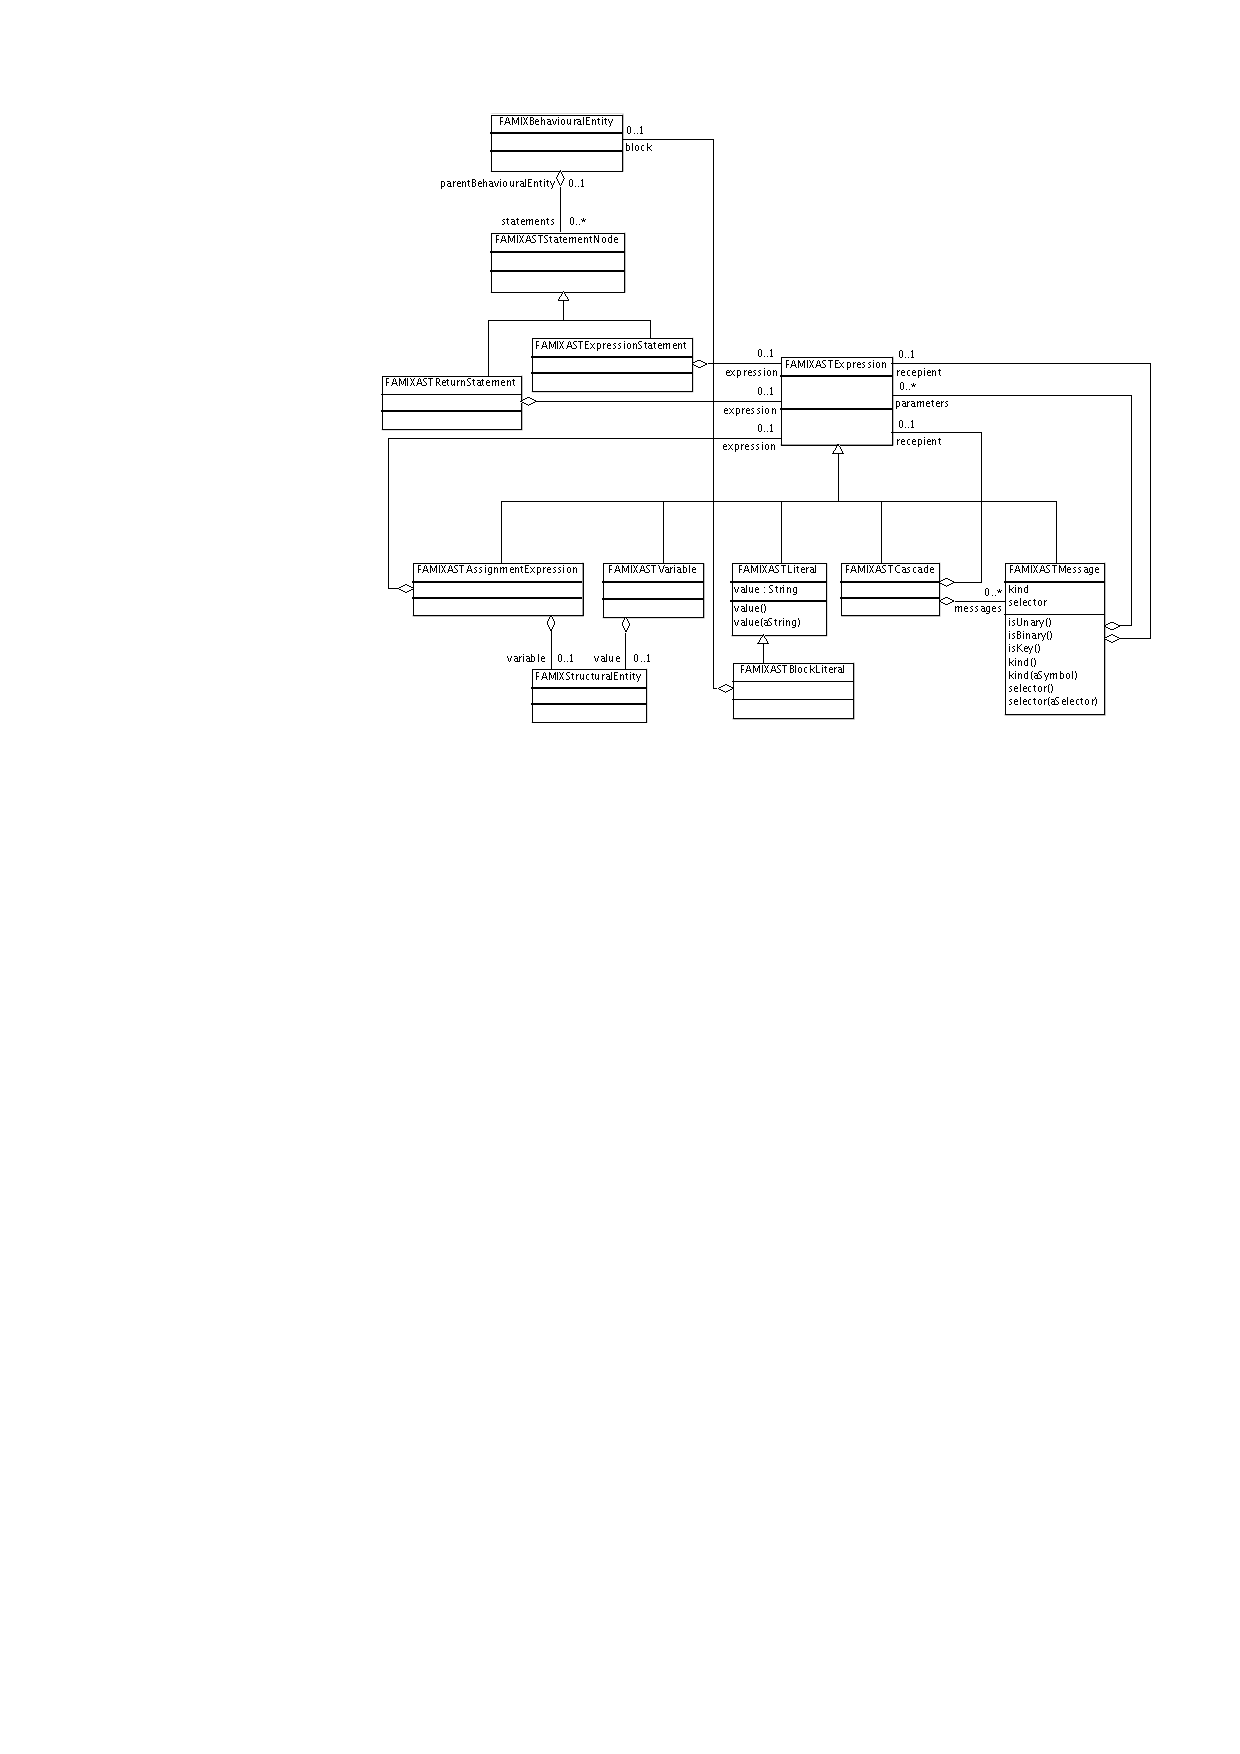
\includegraphics[width=0.95\textwidth]{SmalltalkASTClassDiagram}
  \caption{Діаграма FAST для смолтоку\label{smtFast}}
\end{figure}

Як видно з діаграми, в моделі FAST для смолтоку не тільки присутні ланки, які непритаманні для цієї мови, але й деякі деталі змодельовані не так, як це реалізовано в дереві браузера для рефакторингу.

Перш за все в цій моделі присутня ланка FASTStatementBlock, яка являє собою набір речень. В C--подібних мовах ця структура обмежена фігурними дужками і є тілом методів, а також часто зустрічається як тіло інструкцій if, for, while та подібних. В смолтоці нічого подібного немає, але нам набагато легше мати зайвий прошарок, який можна оминути, чим потім робити великі зміни при адаптації C--подібних мов. Через цей нюанс в FASTBehaviouralEntity визначений метод \emph{statement}, який повертає всі речення з блоку речень. Таким чином ми можемо доступитись до речень безпосередньо із сутності з поведінкою.

Також в смолтоці немає речень як таких. Абстрактне синтаксичне дерево браузера для рефакторингу містить просто визначення ланки повернення і ланки зі значенням на одному рівні з ланками методу та прагми. Так як смолток не є строго--типізованою мовою, то в ній не важливо будувати важкі ієрархії лише для того, щоб взірці різних класів могли знаходитись в одній колекції. Натомість середовище Moose передбачає щось в стилі строгої типізації, адже прагми, які визначають властивості та зв'язки між ланками моделі, вказують тип цих зв'язків. Тим не менше ця концепція гарно вписується в синтаксис смолтоку, і тому в нас присутні два типи речень: речення з виразом, та речення повернення з методу.

Щодо відмінності від моделі дерева у браузері для рефакторингу, то вона проявляється у структурі каскадного повідомлення. Оригінально каскадне повідомлення містило набір повідомлень, перше з яких містило отримувача, як показано на рис.~\ref{rbCascade}.
\begin{figure}[h]
        \vspace{\columnsep}
        \centering
        \begin{subfigure}[b]{0.45\textwidth}
                \centering
                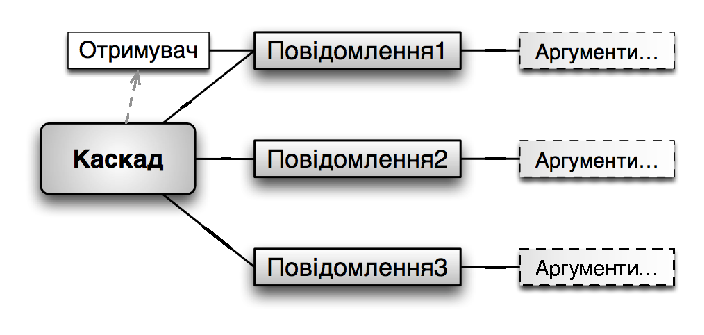
\includegraphics[width=\textwidth]{rbCascade}
                \caption{Браузер рефакторингу\label{rbCascade}}
        \end{subfigure}
        \hspace{0.05\textwidth}
        \begin{subfigure}[b]{0.45\textwidth}
                \centering
                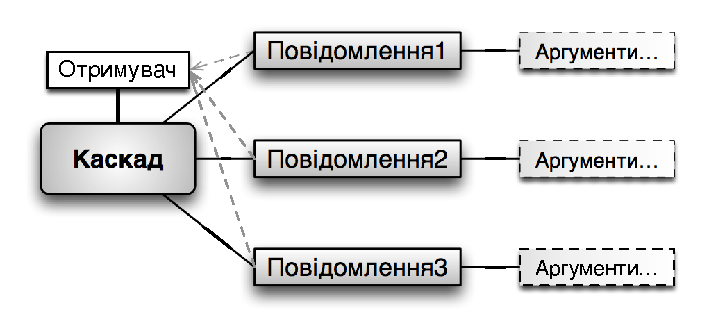
\includegraphics[width=\textwidth]{fastCascade}
                \caption{FAST\label{fastCascade}}
        \end{subfigure}
        \caption{Порівняння реалізацій моделі каскадного повідомлення}
\end{figure}
Штриховою лінією показано, що каскад має непрямий доступ до отримувача через перше повідомлення. Натомість у FAST отримувач безпосередньо зв'язаний з ланкою каскаду і всі повідомлення мають до нього непрямий доступ через каскад (рис.~\ref{fastCascade}). Перш за все це накладає одинакові умови на повідомлення --- всі вони не мають безпосереднього отримувача. Крім того така модель природніша для сприйняття, оскільки каскадне повідомлення являє собою набір повідомлень, які надсилаються до одного і того ж об'єкту,

Можна також звернути увагу на особливість реалізації зворотнього зв'язку іменованої сутності. Як було згадано в основних ідеях FAST, ми хочемо мати зв'язок з батьківським ланками. Проблема полягає у „строгій типізації“ яку накладає платформа Moose. В іменованої сутності уже є зв'язок з батьківським виразом--іменованої сутності, але вона також може бути дочірньою ланкою виразу--присвоєння. Тому в іменованої сутності присутній ще один зворотній зв'язок з ланкою типу виразу--присвоєння. Таким чином, аналізуючи певну іменовану сутність ми можемо зразу сказати де вона використовується, а також перейти вверх по ієрархії ланок. 

\subsection{Спосіб створення моделі з вихідного коду}
Оригінально з метою створення FAST--моделі з вихідного коду, використовувався парсер браузеру для рефакторингу, який по замовчуванню присутній у Pharo. Згодом, коли для роботи з Java почав використовуватись PetitParser, генерацію моделі із Smalltalk було переведено на використання тієї ж технології. Результат роботи PetitParser для Smalltalk був ідентичний до результату парсера браузера для рефакторингу, але при використання однакової технології в різних вітках цього проекту, дозволяє досягнути кращої якості. Також перехід між персерами включав в себе зміну типу вхідних даних. В оригінальній реалізації використовувався скомпільований метод. В новій версії для генерації моделі використовувався безпосередньо текстовий рядок з вихідним кодом методу. Завдяки цього можна знову ж таки досягнути кращої єдиності реалізації даної системи, так як робота із байткодом Smalltalk притаманна лише для цієї мови. На противагу, вихідний код у вигляді текстового рядка доступний для кожної мови програмування.

\clearpage

\section{Метамодель абстрактного дерева Java}

З моделлю Java працювати набагато важче, так як вона містить набагато більше ланок. Сама граматика Java містить в три рази більше ланок чим граматика Smalltalk \cite{meet-grammars}. Відповідно, ланок абстрактного синтаксичного дерева також в кілька разів більше. Наприклад, у Java шістнадцять типів речень, в той час, як у Smalltalk їх лише два. Щодо типів виразів, то у Java їх близько тридцяти, на відміну від п'ятнадцяти у Smalltalk. Через брак часу було прийняте рішення лише вибірково реалізувати певні ланки дерева, наявність яких, дасть можливість перевірити роботу алгоритмів, попередньо реалізованих для моделі Smalltalk. Як показує практика, дуже важко передбачити всі можливі випадки, які можуть виникнути при моделюванні мов програмування. Тому найкращим рішенням є просування маленькими кроками, перевірка сумісності, відладка і перехід до наступної ітерації.

\subsection{Структура моделі}
Базова структура включає в себе:
\begin{itemize}
  \item ланку методу;
  \item примітивні речення такі як повернення, та речення--вираз;
  \item речення--цикл, в конкретному випадку while;
  \item речення--галуження: if;
  \item речення, яке визначає нові змінні
  \item цілочисельні, булівські, та рядкові літерали;
  \item інфіксну операцію.
\end{itemize}

Так, як речення циклу та галуження може містити нові простори імен, то це дозволить перевірити алгоритм, який проводить розв'язку символів. Також ці речення змінюють цикломатичну складність методу, що допоможе перевірити алгоритм, який обчислює цю метрику. 

\subsection{Спосіб створення моделі з вихідного коду}
Як і для смолтоку, модель абстрактного синтаксичного дерева Java потрібно будувати на вимогу, маючи в наявності вихідний код. Першим способом реалізації було розширення та використання програми VerveineJ. На даний момент саме вона використовується для побудови FAMIX моделей з вихідних файлів Java. Позитивними частинами цієї програми є використання нею JDT (Java Development Tools) бібліотеки середовища Eclipse, що значно полегшує генерацію абстрактного синтаксичного дерева джави з вихідного коду. Варто зауважити, що JDT генерує абстрактне синтаксичне дерево за специфікаціями Oracle, тому в подальшому його потрібно перетворити у FAST. Щодо поганих сторін такого підходу, то спочатку модель зберігається зовнішньою джава--програмою у форматі MSE, а тоді вже читається середовищем Moose і перетворюється у FAMIX модель. Очевидно, що робота з проміжним форматом вже передбачає в собі слабке місце. Крім того використання зовнішньої джава програми означає залежність на JRE середовищі, наявності самої програми, а також функціональності бібліотек OSProces, які дозволяють викликати зовнішні скрипти з Фаро. Також розробка на двох різних платформах несе додаткове навантаження, так як приходиться доволі часто змінювати спосіб мислення щодо написання коду.

З другого боку на момент здійснення вибору вже існувала часткова реалізація парсера вихідного коду Java розроблена на основі PetitParser. Ця реалізація в собі включала повний лексикон та синтаксис Java з тестами, а також частково реалізований парсер. Отже для використання цього парсера, щоб завантажувати FAST, передбачало ще й роботу над самим парсером. Тим не менше цей варіант був найкращим оскільки він використовував технології, які були застосовані в ланцюжку інструментів FAST для роботи із Smalltalk. Таким чином використання PetitParser для всіх віток моделей FAST означає, що весь час призначений для покращення парсера не буде розпорошуватись на декілька технологій, а буде зосереджений безпосередньо на одній. Аналогічно у цьому підході відсутні всі негативні сторони VerveineJ.

\clearpage

\section{Symbol resolution}
При генерації абстрактного синтаксичного дерева з вихідного коду в якості листків графу ми можемо отримати \emph{іменовані сутності} або ж літерали. Іменована сутність несе лише інформацію про назву змінної чи класу і цього доволі мало для аналізу вихідного коду. Однаковий ідентифікатор може зустрічатись в багатьох місцях програми, але відноситись до різних змінних. Для того, щоб визначити які сутності відносяться до тієї самої змінної будемо використовувати \textbf{область визначення (scope)} змінної, а також метазмінну яка буде знаходитись в цій області, і буде зв'язана з іменованими сутностями абстрактного синтаксичного дерева. Кожна область буде мати батьківську область визначення. Для методу це будуть змінні класу. Для класу - змінні пакету. Таким чином при пошуку змінної з певним ім'ям, якщо ми не знайдемо її в поточній області визначення, то зможемо продовжити пошуки в батьківській. Головне завдання об'єкту області визначення:
\begin{enumerate}
\item знаходити метазмінну за відповідною назвою.
\item додати метазмінну з відповідною назвою
\item повернути сутність до якої ця область прив'язана. Наприклад: метод, клас, блок
\end{enumerate}

Перший пункт реалізується дуже легко. Для збереження інформації про взаємозв'язок назв і сутностей метазмінних використовується просто словник в якому кожній назві відповідає певна змінна. На наступному прикладі можна детальніше розглянути, як працює даний метод:
\begin{lstlisting}[language=Smalltalk]
FAMIXScope>>resolve: name
	^ variables
		at: name
		ifAbsent: 
			[parent notNil 
				ifTrue: [parent resolve: name] 
				ifFalse: nil]
\end{lstlisting}
Все зводиться до отримання значення за ключем--назвою змінної. Якщо такого немає, то питаємо в батьківської області.

Другий пункт зводиться до занесення пари ключ--значення у словник. А третій пункт передбачає змінну взірця класу, яка буде вказувати на власника області, та отримувач і встановлювач змінної.

В якості метазмінних використовуються сутності змінних визначені у FAMIX. Перш за все вони вже мають необхідну метаінформацію, але крім того деякі моделі під час генерації частково виконують резолюцію символів. Таким чином ми можемо використати вже зроблену роботу.

В сутностей, які мають області визначення повинен бути метод для отримання цієї області. Пропонується використовувати ліниву ініціалізацію, так як деякі частини фамікс вже розв'язують проблему ідентифікації змінної. Таким чином у момент часу, коли комусь потрібно отримати область визначення, її вже можна буде наповнити деякими метазмінними. Для прикладу розглянемо реалізацію такої лінивої ініціалізації для сутності методу моделі FAMIX:
\begin{lstlisting}[language=Smalltalk]
FAMIXMethod>>scope
	^ self privateState cacheAt: #fastScope ifAbsentPut: [
		| scope |
		scope := FASTScope newWithParent: self belongsTo scope.
		scope owner: self.
		self implicitVariables do: [:variable | scope add: variable].
		self parameters        do: [:variable | scope add: variable].
		self localVariables    do: [:variable | scope add: variable].
		scope]
\end{lstlisting}

Перш за все варто зауважити, що ми додаємо цей функціонал до класу зробленого кимсь іншим. Це ще одна позитивна сторона цього підходу, так як ми хочемо мати можливість застосовувати наш алгоритм до вже існуючих моделей, а не будувати все з нуля. Відповідно область визначення зберігається в приватному стані MooseEntity, але якщо ми хочемо отримати область вперше, то нам потрібно перш за все її створити та ініціалізувати. Цей метод створює область визначення зразу з батьківською областю, яка отримується від батька поточної сутності. Далі сутність встановлює себе як власника області, і додає в неї всі неявні та локальні змінні а також параметри. Таким чином, якщо на момент отримання області вже були якісь дані про змінні в даній сутності --- вони будуть скопійовані в область.

Щодо самого алгоритму резолюції символів, то він зводиться до відвідування моделі FAST та запитування поточної області про метазмінну з даним ім'ям. Ось короткий приклад, як це зроблено в смолтоці:
\begin{lstlisting}[language=Smalltalk]
FASTResolutionVisitor>>acceptNamedEntityNode: aNamedEntityNode
	aNamedEntityNode famixVariable: (scope resolve: aNamedEntityNode name)
\end{lstlisting}

При отриманні відвідувачем ланки яка є іменованою сутністю, він їй в якості метазмінної, присвоює результат виконання методу \lstinline$resolve:$ поточної області. Також можливі деякі модифікації, наприклад, створення „накопичуючої“ області, яка буде створювати нову змінну при її її відсутності. Таку область можна зробити найстаршою в ланцюжку батьківства. Таким чином в ній будуть накопичуватись неоголошені змінні. Аналогічно для скриптових мов програмування в яких немає явного оголошення змінних --- області повинні створювати змінні при першій їх появі.
\clearpage

\section{Метрики коду}
Маючи абстрактне синтаксичне дерево, дуже зручно обчислювати на ньому метрики. Так як наше синтаксичне дерево доволі абстрактне, то реалізувавши на ньому обчислення метрик коду, ми зможемо адаптувати алгоритм до різних мов програмування, моделей. 

Одною з найпростіших метрик є кількість \emph{речень} коду. Так як кожна сутність з поведінкою має в собі колекцію \emph{речень}, то весь алгоритм зводиться до обчислення розміру колекції, що вміє зробити сама колекція.

\subsection{Цикломатична складність}
Цикломатичною складністю вважається кількість можливих шляхів виконання коду. Наприклад, якщо програма не містить ніяких інструкцій галуження та циклів, то її можна пройти одним чином. Цикломатична складність такої програми рівна 1. Якщо ж в програмі з'явиться одна інструкція галуження (\lstinline$if$), то її вже можна буде пройти двома способами. Це результує у цикломатичній складності 2. Аналогічне правило діє на циклах. 

Правило обчислення цикломатичної складності каже, що вона дорівнює кількості інструкцій галуження та циклів плюс 1. В такому випадку алгоритм буде еквівалентний відвідуванню дерева. При цьому при отриманні ланки, яка збільшує цикломатичну складність --- збільшувати змінну взірця на 1. Цей алгоритм дозволяє враховувати навіть такі екзотичні випадки як інструкція циклу, що має альтернативний блок else у мові програмування Python. Така інструкція збільшує цикломатичну складність програми на 2. Але ця особливість зводиться лише до визначення чергової дії відвідувача на отримання певної ланки абстрактного синтаксичного дерева.

Проблеми починаються у мовах з лямбда--функціями, блоками та замиканнями. Найкращим прикладом є, звичайно ж, Смолток. В цій мові програмування інструкції циклів та галуження взагалі відсутні. На жаль в такому випадку важко сказати, чи конкретне повідомлення буде збільшувати цикломатичну складність, чи ні. Ми не знаємо якому саме об'єкту буде надіслано повідомлення, відповідно і не знаємо реалізацію. З цією метою будемо використовувати метод аналогічний до того, що використовується в середовищі Moose. Визначимо дві множини селекторів: галуження і циклів та додамо туди наперед відомі селектори, такі як \lstinline$ifTrue:ifFalse:$, \lstinline$whileTrue:$, \lstinline$detect:ifNone:$. Тоді при визначенні чи повідомлення збільшує цикломатичну складність будемо перевіряти, чи воно присутнє в тій чи іншій колекції. Варто звернути додаткову увагу на використання двох колекцій, а не одної. Селектор \lstinline$detect:ifNone:$ повинен бути в обох колекціях, так як його реалізація включає в себе як цикл так і галуження. Тому при при визначенні цикломатичної складності, він буде виявлений в обох колекціях, і тому збільшить складність на 2 \cite{cyclocomplexity-moose}.

\subsubsection{Удосконалення алгоритму відвідувача}
Як вже було описано вище --- алгоритм зводиться до відвідування ланок дерева, і при опрацюванні тої чи іншої ланки додавання збільшення загальної цикломатичної складності в залежності від певних умов, скажімо типу селектора. Але це означає, що для кожної особливої ланки нам потрібно буде перевизначати поведінку відвідувача. Натомість цю логіку можна перенести всередину самого об'єкту. Нехай будь яка ланка, яка відповідає певному вихідному коду буде знати свій внесок у цикломатичну складність. У FAMIX такій ланці відповідає клас FAMIXSourcedEntity. В ньому ми можемо визначити метод \emph{cyclomaticComplexityContribution}, який буде повертати 0. Тоді для кожного класу, який буде відображати ланку, що впливає на цикломатичну складність, цей метод буде перевизначатись. Наприклад для інструкцій if, for, while в мові джава цей метод буде повертати 1. Для інструкції for ... else в мові Python, цей метод буде повертати 2, так як вона об'єднує в собі цикл і галуження. Для повідомлень у смолтоці цей метод буде обчислювати внесок складності динамічно, адже він буде залежати від селектора повідомлення. Ще одним плюсом цього методу є можливість кешування обчислених даних в самій ланці, таким чином їх не треба буде перераховувати всі наступні рази. Також внесок цикломатичної складності можна зробити властивістю ланки, що дозволить переглядати цю інформацію в панелі середовища Moose.

\clearpage

\section{Охорона праці та безпеки в надзвичайних ситуаціях}

\subsection{Вступ}
З розвитком науково-технічного прогресу важливу роль грає можливість безпечного виконання людьми своїх трудових обов'язків.
Охорона здоров'я людей що працюють, забезпечення безпеки умов праці, ліквідація професійних захворювань і виробничого травматизму становить основу людської безпеки. Проте не варто забувати, що небезпечні чинники можуть діяти на людський організм не-поодинці, а взаємопов’язано. Але нажаль ми не можемо проаналізувати всі можливі комбінації сукупної дії небезпечних та шкідливих чинників. Невід’ємним елементом сьогодення є те, що людина проводить половину свого дня у приміщені за роботою.
Мета роботи – вивчення безпеки праці на робочому місці, вплив шкідливих чинників на працюючу особу й відчуття міри захисту від неї.
У зв’язку з цим була створена та розвивається наука про безпеку праці та життєдіяльності людини. Це комплекс заходів, вкладених у забезпечення безпеки людини у середовище проживання, збереження здоров'я, розробку методів і засобів захисту за методом зниження впливу шкідливих і найнебезпечніших чинників до допустимих значень, вироблення заходів для обмеження шкоди та ліквідацію наслідків надзвичайних ситуацій мирного й військової часу.
Під час виконання бакалаврської роботи було використано ряд різноманітного приладдя яке дає змогу опрацьовувати низку матеріалу, а саме комп’ютери, принтери, сканери. Не враховуючи приміщення в якому відбувається цей тривалий процес, а саме лабораторії, комп’ютерні класи
За умов роботи з ПК виникають наступні небезпечні та шкідливі чинники: несприятливі мікрокліматичні умови, освітлення, електромагнітні випромінювання, забруднення повітря шкідливими речовинами (джерелом яких може бути принтер, сканер), шум, вібрація, електричний струм, електростатичне поле, напруженість трудового процесу .


\subsection{Аналіз стану умов праці}
\subsubsection{Характеристика виробничого середовища та чинників трудового процесу}
\begin{itemize}
\item Магістерська робота виконувалась і оформлювалась у студентській лабораторії, яка знаходиться у приміщенні ЛНУ ім. І. Франка на філософському факультеті кафедрі психології 1А. Вул. Дорошенка 41.
\item Приміщення планово-економічного відділу розташовано на третьому поверсі п'ятиповерхового будинку. У приміщенні розташовано 3 робочих місць з комп’ютерами. Розміри даного приміщень складають: довжина – 10 м, ширина – 6 м, висота – 3,5 м, тобто загальна фактична площа складає 60 м2.
\item Необхідна площа на 3 робочих місця із установленими ПК складає 18 м2, що не перевищує фактичну. Обсяг кабінету на одного працюючого складає 70.м3, отже відповідає нормі (ДНАОП 0.00-1.31-99) [3] – не менше 20 м3. Площа одного робочого місця з відео дисплейним терміналом повинна бути не менше 6 м. кв, а об’єм не менше 20м.кб. Робочі місця розташовані від стіни з вікнами 1.5 м. а від бокових стін 1 м. Відстані між боковими поверхнями відео дисплеїв 1.2 м, а від тильного боку одного до екрану другого 2.5 м( я не знаю точно як порахувати на 10 робочих мість)(в цьому розділі  не наводьте нормативів, лише  те що реально  є. Це можна видалити)
\item Загальна кількість робочих місць 10.
\item Приміщення розташоване з північно-західною орієнтацією вікон. Мікроклімат у приміщенні забезпечує комфортне самопочуття людини. Оптимальна температура в приміщені становить: в теплий період року 23–25 °С, у холодний 22–24 °С. Відносна вологість повітря коливається в межах 60-40 \%. Швидкість руху повітря не перевищує 0.2 м/с – у теплий період часу, а у холодний 0.1 м/с. Приміщення з відеодисплейним терміналом оснащене припливно-витяжною вентиляцією та забезпечене природним вентилюванням.
\item Освітлення приміщення змішане: природне і штучне. При цьому коефіцієнт природного освітлення не менше 1,5 \%, освітленість при штучному освітлені в площині робочої поверхні становить 300-500лК. Також допускається локальне освітлення з освітленістю екрана не більше 300 лК.
\item У даному приміщені не має наявних хімічних речовин. Основним джерелом небезпек під час роботи з персональним комп’ютером є відеодисплейний термінал на основі електронно-променевої трубки. Більш безпечні відеодисплейні термінали з плазмовими та рідинно-кристалічними екранами. Крім безпосереднього впливу на організм людини, робота відеодисплейних терміналів має ще й опосередкований вплив, а саме: зумовлює порушення балансу аероіонів у зоні дихання користувача і призводить до зменшення кількості від’ємних аероіонів, які мають суттєвий вплив на імунну систему організму. Пониження імунітету людини внаслідок зменшення негативних аероіонів зумовлює інші порушення в організмі, зокрема й тих, що непов’язані з роботою на персональному комп’ютері.
\item У приміщені наявна аптечка. 
\item До засобів гасіння пожеж належать встановлені пожежні стволи, внутрішні пожежні водопроводи, вогнегасники, сухий пісок, азбестові ковдри. Пожежні крани встановлені в коридорах, на сходових клітках та вході. Приміщення забезпечені вогнегасниками. Для виявлення стадії загоряння та оповіщення використовують системи автоматичної пожежної сигналізації.
\item На робочому місці викладачі проводять повний інструктаж з  охорони праці, повідомлять де розміщені плани будівлі, додаткові входи і виходи, розміщення вогнегасників. Також повідомлять про ряд небезпечних речовин та чинників, що впливають на наш організм.
\end{itemize}
\subsubsection{Опис трудового процесу} 
Негативний вплив на організм людини виникає через неадекватне (надто велике або надто мале) навантаження на окремі системи організму. Такі перекоси у напруженні різних систем організму, що трапляються підчас роботи з відеодисплейним терміналом, зокрема, значна напруженість зорового аналізатора і довготривале малорухоме положення перед екраном, не тільки не зменшують загального напруження, а навпаки, призводять до його посилення і прояву стресових реакцій.
Виконання бакалаврської роботи належить до легких робіт згідно класифікації робіт за ступенем важкості.
Основним робочим становищем є положення сидячи. Робоча поза сидячи викликає мінімальне стомлення людини. Раціональне планування робочого місця передбачає чіткий лад і сталість розміщення предметів. Те, що потрібно виконувати частіше, лежить у зоні легкої досяжності робочого простору. 
Можна вважати, що робоче місце досить добре пристосоване для ефективного виконання поставлених завдань і не приводить до погіршення продуктивності праці та погіршення самопочуття чи здоров’я.
\subsubsection{Аналіз методів дослідження, обладнання та характеристика речовин}
Під час виконання бакалаврської роботи. використовують персональні комп’ютери та периферійні пристрої (лазерні та струменеві друки, копіювальну техніку, сканери). Негативний вплив цих пристроїв на організм людини виникає через неадекватне (надто велике або надто мале) навантаження на окремі системи організму. Такі перекоси у напруженні різних систем організму, що трапляються під час роботи з ПК, зокрема, значна напруженість зорового аналізатора і довготривале малорухоме положення перед екраном, не тільки не зменшують загального напруження, а навпаки, призводять до його посилення і прояву стресових реакцій. Найбільшому ризику виникнення різноманітних порушень піддаються: органи зору, м’язово-скелетна система, нервово-психічна діяльність, репродуктивна функція у жінок.
Робота з комп’ютером характеризується значною розумовою напругою і нервово-емоційним навантаженням, високою напруженістю зорової праці та досить великим навантаженням на м’язи рук під час роботи з клавіатурою.
У процесі роботи з комп'ютером необхідно дотримуватися правильного режиму праці та відпочинку. Інакше у людини відзначаються значна емоційна напруга зорового апарату, що може призвести до появи головного білю, дратівливості, порушення сну, почуття виснаження. Раціональний режим праці та відпочинку передбачає запровадження регламентованих перерв, рівномірний розподіл навантаження протягом робочого дня, регулярні комплекси вправ для очей, рук, хребта для  поліпшення мозкового кругообігу та психофізіологічного розвантаження.
З метою запобігання перевантаження організму як в цілому, так і окремих його функціональних систем, передусім зорового та рухового аналізаторів, центральної нервової системи, загальний час щоденної роботи з відеодисплейним терміналом треба обмежити чотирма годинами та обов’язково дотримуватись регламентованих перерв.
Робота з ПК супроводжується також виділенням значної кількості тепла, шуму, вібрації та електромагнітних випромінювань.

\subsection{Організаційно-технічні заходи}
\subsubsection{Організація робочого місця і роботи}
Санітарно-гігієнічні та ергономічні вимоги до параметрів робочого місця, розміщення обладнання, пристроїв та персонального комп’ютера на ньому, психофізіологічні особливості праці (напруженість трудового процесу).
Робоче місце – це зона трудових дій працівника, обладнана для виконання певних операцій виробничого процесу, де взаємодіють три головні елементи праці – предмет, засоби і суб’єкт праці. На одному робочому місці можуть працювати два або кілька працівників, які виконують спільне завдання.  Наукова організація робочого місця передбачає створення працівникові всіх необхідних умов для високопродуктивної і високоякісної праці за можливо менших фізичних зусиль і мінімальному нервовому напруженні та передбачає:
\begin{itemize}
\item оснащеність робочого місця відповідним основним і допоміжним устаткуванням, технологічною і організаційною оснасткою;
\item раціональне планування, тобто найзручніше і найефективніше розміщення усіх елементів робочого місця для трудового процесу;
\item створення безпечних і здорових умов праці.
Просторова організація робочого місця повинна забезпечувати:
\item відповідність планування робочого місця санітарним і протипожежним нормам і вимогам;
\item безпеку працівникам;
\item відповідність просторових відношень між елементами робочого місця, антропометричними, біомеханічними, фізіологічними, психофізіологічними і психічними можливостями людини, що працює;
\item можливість виконання основних і допоміжних операцій в робочому положенні, що відповідає специфіці трудового процесу, в раціональній робочій позі і з використанням найбільш ефективних прийомів праці;
\item вільне переміщення працівника за оптимальними траєкторіями;
\item достатню площу для розміщення обладнання, інструменту, засобів контролю, деталей та ін.
Просторові та розмірні співвідношення між елементами робочого місця повинні дозволяти:
\item розміщення працівника з врахуванням робочих рухів і переміщень згідно з технологічним процесом;
\item оптимальний огляд джерела візуальної інформації;
\item зміну робочої пози і положення;
\item раціональне розміщення основних і допоміжних засобів праці.
\end{itemize}
Обов’язковою умовою є те, що на робочому місці повинні знаходитись лише ті технічні засоби, які необхідні для виконання робочого завдання, і розміщуватися вони повинні в межах досяжності з метою виключення частих нахилів і поворотів корпусу людини, що працює.
Під час роботи з персональним комп’ютером повинні бути дотримані наступні вимоги.
Вимоги до приміщення. Площу приміщень, в яких розташовують персональні комп’ютери, визначають згідно з чинними нормативними документами з розрахунку на одне робоче місце, обладнане ПК:
\begin{itemize}
\item площа — не менше 6,0 м2;
\item об’єм — не менше 20,0 м3, з урахуванням максимальної кількості осіб, які одночасно працюють у зміні;
\item робочі місця повинні бути розташовані на відстані не менше ніж 1 м від стіни з вікном;
\item відстань між бічними поверхнями комп’ютерів має бути не меншою за 1,2 м;
\item відстань між тильною поверхнею одного комп’ютера та екраном іншого не повинна бути меншою 2,5 м;
\end{itemize}
Прохід між рядами робочих місць має бути не меншим 1 м.
Користування ПК є основним видом діяльності, то ПК і його периферійні пристрої (принтер, сканер) розміщується на основному робочому столі, як правило, з лівого боку.
Вимоги до організації робочого місця з ПК. Конструкція робочого місця користувача ПК має забезпечувати підтримання оптимальної робочої пози з такими ергономічними характеристиками: 
\begin{itemize}
\item ступні ніг — на підлозі або на підставці для ніг; 
\item стегна — в горизонтальній площині; 
\item передпліччя — вертикально; 
\item лікті — під кутом 70–90° до вертикальної площини; 
\item зап’ястя зігнуті під кутом не більше 20° відносно горизонтальної площини; 
\item нахил голови — 15–20° відносно вертикальної площини.
\end{itemize}
Якщо користування ПК є основним видом діяльності, то ПК і його периферійні пристрої (принтер, сканер) розміщується на основному робочому столі, як правило, з лівого боку. Якщо використання ПК є періодичним, то він, як правило, розміщується на приставному столі, переважно з лівого боку від основного робочого столу.
Кут між поздовжніми осями основного та приставного столів має бути 90–140°.
Висота робочої поверхні столу для ПК має бути в межах 680–800 мм, а ширина — забезпечувати можливість виконання операцій в зоні досяжності моторного поля.
Рекомендовані розміри столу: висота 725 мм, ширина 600–1400 мм, глибина 800–1000 мм.
Робочий стіл для ПК повинен мати простір для ніг висотою не менше 600 мм, шириною не менше 500 мм, глибиною на рівні колін не менше 450 мм, на рівні витягнутої ноги — не менше 650 мм.
Робочий стіл для ПК, як правило, має бути обладнаним підставкою для ніг шириною не менше 300 мм та глибиною не менше 400 мм, з можливістю регулювання по висоті в межах 150 мм та кута нахилу опорної поверхні - в межах 20°. Підставка повинна мати рифлену поверхню та бортик на передньому краї заввишки 10 мм. Застосування підставки для ніг тими, у кого ноги не дістають до підлоги, є обов’язковим.
Робоче сидіння (сидіння, стілець, крісло) користувача ПК повинно мати такі основні елементи: сидіння, спинку, стаціонарні або знімні підлокітники. У конструкцію сидіння можуть бути введені додаткові елементи, що не є обов’язковими: підголовник та підставка для ніг. 
Робоче сидіння користувача ПК повинно бути підйомно-поворотним, таким, що регулюється за висотою, кутом нахилу сидіння та спинки, за відстанню спинки до переднього краю сидіння, висотою підлокітників. Регулювання кожного параметра має бути незалежним, плавним або ступінчатим, мати надійну фіксацію.
Хід ступінчатого регулювання елементів сидіння має становити для лінійних розмірів 15–20 мм, для кутових – 2–5°. Зусилля під час регулювання не повинні перевищувати 20 Н. Ширина та глибина сидіння повинні бути не меншими за 400 мм. Висота поверхні сидіння має регулюватися в межах 400–500 мм, а кут нахилу поверхні - від 15° вперед до 5° назад. Поверхня сидіння має бути плоскою, передній край - заокругленим. Висота спинки сидіння має становити 300±20 мм, ширина - не менше 380 мм, радіус кривизни в горизонтальній площині - 400 мм. Кут нахилу спинки повинен регулюватися в межах 0–30° відносно вертикального положення. Відстань від спинки до переднього краю сидіння повинна регулюватись у межах 260–400 мм.
Для зниження статичного напруження м’язів рук необхідно застосовувати стаціонарні або знімні підлокітники довжиною не менше 250 мм, шириною 50–70 мм, що регулюються по висоті над сидінням у межах 230±30 мм та по відстані між підлокітниками в межах 350–500 мм.
Поверхня сидіння, спинки та підлокітників має бути напівм’якою, з неслизьким, ненаелектризовувальним, повітронепроникним покриттям та забезпечувати можливість чищення від бруду.
Монітор та клавіатура мають розташовуватися на оптимальній відстані від очей користувача, але не ближче 600 мм, з урахуванням розміру алфавітно-цифрових знаків та символів.
Розташування монітору має забезпечувати зручність зорового спостереження у вертикальній площині під кутом ±30° від лінії зору працівника.
Клавіатуру слід розміщувати на поверхні столу або на спеціальній, регульованій за висотою, робочій поверхні окремо від столу на відстані 100–300 мм від краю, ближчого до працівника. Кут нахилу клавіатури має бути в межах 5–15°.
Розміщення принтера або іншого пристрою введення-виведення інформації на робочому місці має забезпечувати добру видимість монітору, зручність ручного керування пристроєм введення-виведення інформації в зоні досяжності моторного поля: по висоті 900–1300 мм, по глибині 400–500 мм.
При потребі високої концентрації уваги під час виконання робіт з високим рівнем напруженості суміжні робочі місця з ПК необхідно відділяти одне від одного перегородками висотою 1,5–2 м.
Режим праці та відпочинку користувачів ПК встановлюють з урахуванням психофізіологічної напруженості їхньої праці, динаміки функціонального стану систем організму та працездатності. Раціональний режим праці та відпочинку передбачає запровадження регламентованих перерв, рівномірний розподіл навантажень протягом робочого дня, регулярні комплекси вправ для очей, рук, хребта, поліпшення мозкового кругообігу та психофізіологічне розвантаження.
З метою запобігання перевантаження організму як в цілому, так і окремих його функціональних систем, передусім зорового та рухового аналізаторів, центральної нервової системи, загальний час щоденної роботи з ПК обмежують. Робота з персональним комп’ютером вважається основною, якщо вона займає не менше як 50 % часу робочого дня чи робочої зміни.
З урахуванням характеру трудової діяльності, напруженості та важкості праці з використанням ПК під час основної роботи за восьмигодинної робочої зміни встановлюють додаткові регламентовані перерви:
\begin{itemize}
\item для розробників програм тривалістю 15 хв через кожну годину роботи;
\item для операторів персональних комп’ютерів тривалістю 15 хв через дві години роботи;
\item для операторів комп’ютерного набору тривалістю 10 хв через кожну годину роботи.
\end{itemize}
За жодних умов безперервна робота з ПК не повинна перевищувати чотири години.
За дванадцятигодинної робочої зміни протягом перших восьми годин регламентовані перерви встановлюють аналогічно до восьмигодинної робочої зміни, а протягом останніх чотирьох годин тривалістю 15 хв через кожну годину незалежно від характеру трудової діяльності.

Навчання та інструктажі з безпеки праці. Перед допуском до самостійної роботи кожен працівник має право на навчання з питань охорони праці і роботодавець зобов’язаний провести таке навчання у вигляді двох інструктажів з питань охорони праці:
\begin{itemize}
\item вступного, який проводять працівники служби охорони праці об’єкта господарювання з усіма працівниками, яких приймають на роботу незалежно від їхньої освіти та стажу роботи за програмою, в якій подають загальні питання охорони праці із врахуванням її особливостей на об’єкті господарювання;
\item первинного, який проводять керівники структурних підрозділів на робочому місці з кожним працівником до початку їхньої роботи на цьому робочому місці.
\end{itemize}
Проходження цих інструктажів з питань охорони праці підтверджується записами у відповідних журналах обліку інструктажів і скріплюється підписами осіб, які проводили інструктажі та осіб, які отримали інструктажі.
Організаційні заходи перед початком, під час і після завершення роботи.
Працівники до початку роботи повинні перевірити візуально наявність і справність електрообладнання та його заземлення, а під час виконання роботи не залишати без нагляду обладнання, яке використовують. Після закінчення роботи необхідно прибрати робоче місце, відключити всі електроприлади від електромережі, перекрити крани водо- та газомережі.

\subsubsection{Санітарно-гігієнічні вимоги до умов праці}
Санітарно-гігієнічні вимоги до умов праці під час виконання роботи описують:
Нормативи з параметрів мікроклімату, освітлення приміщень, рівнів шуму, вібрації та електромагнітних випромінювань.
Мікроклімат виробничих приміщень характеризують температурою, вологістю та  швидкістю руху повітря, а також інтенсивністю радіації, переважно в інфрачервоній та ультрафіолетовій областях спектру електромагнітних випромінювань.
Параметри мікроклімату у приміщеннях повинні забезпечувати комфортне самопочуття організму. Тому у виробничих приміщеннях повинна бути надійна система кліматичного контролю. 
Параметри мікроклімату закритих приміщень нормують санітарні норми ДСН 3.3.6.042‑99. Оптимальні параметри мікроклімату закритих приміщень наведені в таблиці.
Оптимальні параметри мікроклімату закритих приміщень
Категорія
робіт	Температура, ºС	Відносна вологість повітря, %	Швидкість руху повітря, м/с			
холодний період року	теплий період року	холодний період року	теплий період року	холодний період року	теплий період року
Іа	22–24	23–25	60–40	60–40	0,1	0,1
Іб	21–23	22–24	60–40	60–40	0,1	0,2
Освітлення приміщень та робочих місць. Ще один важливий чинник, від якого залежать працездатність і здоров’я людини, – це освітлення. Світло регулює всі функції людського організму і впливає на психологічний стан і настрій, обмін речовин, гормональний фон і розумову активність. 
Найздоровіше освітлення забезпечує природне світло. Його ефективне використання можливе, якщо глибина приміщень не перевищує 6 м. Окрім того, хорошим вирішенням можуть будуть скляні перегородки, що забезпечують зорову і звукову ізоляцію, але в той же час не перешкоджають проникненню природного світла. 
Відносно вікон робоче місце повинно бути розміщено так, щоб природне світло було збоку, переважно з лівого та забезпечувати коефіцієнт природної освітленості не нижче 1,5 \%. Освітленість за штучного освітлення в площині робочої поверхні має становити 300–500 Лк. Якщо таких значень освітленості досягнути не можна, то допускається локальне освітлення, при цьому освітленість екрана не може перевищувати 300 Лк. Відношення яскравості робочих поверхонь не повинно бути більшим ніж 3:1, а яскравості робочих поверхонь і стін (іншого обладнання) - 5:1. Робоче місце, обладнане ПК повинно бути розташоване так, щоб уникнути попадання в очі прямого світла.
Щоб уникнути світлових відблисків від екрану та клавіатури необхідно використовувати комп’ютерне обладнання з матовою поверхнею. Для захисту очей від прямого сонячного світла чи джерел штучного освітлення необхідно застосовувати захисні козирки та жалюзі на вікнах. 
Вимоги до рівнів шуму та вібрації. Шум часто є причиною зниження рівня працездатності, підвищення рівня загальної та професійної захворюваності, частоти виробничих травм. Шум як стрес-чинник є загальнобіологічним подразником, який негативно впливає на всі органи і системи організму. У разі тривалого систематичного впливу шуму може виникнути патологія з переважним ураженням слуху, центральної нервової і серцево-судинної систем.
Гігієнічне нормування рівнів шуму. Допустимі рівні звукового тиску у октавних смугах частот, еквівалентні рівні звуку на робочих місцях встановлені санітарними нормами виробничого шуму, ультразвуку та інфразвуку ДСН 3.3.6.037-99, і для творчої та наукової роботи, навчання, не повинні перевищувати 50 дБА. 
Вібрація приводить тіло і його структурні частини в коливний рух. Розрізняють поперечні, поздовжні і крутильні коливання. За впливом на людину вібрації ділять на місцеві і загальні. Загальні вібрації викликають коливання тіла людини, місцеві – лише окремі частини тіла. Тривала дія вібрацій на організм людини призводить до порушень в центральній нервовій та серцево-судинній системах, погіршує загальний стан людини – появляються втома, головний біль тощо.
Колективні  та індивідуальні засоби і заходи захисту від шкідливого впливу виробничих чинників на здоров’я людини .
Облаштовуючи приміщення для роботи з ПК, потрібно передбачити припливно-витяжну вентиляцію або кондиціювання повітря. Надходження свіжого повітря регулюють, виходячи із таких умов (вказаний об’єм приміщення припадає на одне робоче місце з ПК):
\begin{itemize}
\item	якщо об’єм приміщення 20 м3, то потрібно подати не менш як 30 м3/год повітря;
\item	якщо об’єм приміщення у межах від 20 до 40 м3, то потрібно подати не менш як 20 м3/год повітря;
\item	якщо об’єм приміщення становить понад 40 м3, допускається природна вентиляція, у випадку, коли немає виділення шкідливих речовин.
\end{itemize}
Захист від шуму та вібрацій. Усунення шуму в приміщенні є однією з найскладніших проблем, оскільки джерела шуму різноманітні й потребують комплексу заходів технічного, організаційного і медичного характеру на всіх стадіях проектування, будівництва, експлуатації машин і устаткування. Відомі три головні напрямки зменшення впливу шуму на організм людини:
\begin{itemize}
\item	зменшення рівня шуму у джерелі виникнення, застосування раціональних конструкцій, нових матеріалів і технологічних процесів;
\item	звукоізоляція устаткування за допомогою глушників, резонаторів, кожухів, захисних конструкцій, оздоблення стін, стелі, підлоги тощо;
\item	використання засобів індивідуального захисту.
\end{itemize}
Заходи особистої гігієни на робочому місці (підтримання чистоти, миття лабораторного посуду, рук тощо).
Заходи особистої гігієни на робочому місці передбачають щоденне вологе прибирання, утримання у чистоті робочого місця, наявність на робочому місці тільки необхідних для роботи засобів. На робочому місці необхідно дотримуватись вимог правил внутрішнього розпорядку, зокрема, заборонено приймати їжу, пити, курити та ін.

\subsubsection{Заходи щодо безпеки під час виконання бакалаврської роботи}
1.	Заходи безпеки під час експлуатації персонального комп’ютера та периферійних пристроїв передбачають:
\begin{itemize}
\item	правильну організацію робочого місця та дотримання оптимальних режимів праці та відпочинку під час роботи з ПК;
\item	експлуатацію сертифікованого обладнання;
\item	дотримання заходів електробезпеки;
\item	забезпечення оптимальних параметрів мікроклімату;
\item	забезпечення  раціонального освітлення робочого місця;
\item	зниження рівня шуму та вібрації.
\end{itemize}
2.	Заходи безпеки під час експлуатації інших електричних приладів передбачають дотримання таких правил:
\begin{itemize}
\item	постійно стежити за справним станом електромережі, розподільних щитків, вимикачів, штепсельних розеток, лампових патронів, а також мережевих кабелів живлення, за допомогою яких електроприлади під’єднують до електромережі;
\item	постійно  стежити за справністю ізоляції електромережі та мережевих кабелів, не допускаючи їхньої експлуатації з пошкодженою ізоляцією;
\item	не тягнути за мережевий кабель, щоб витягти вилку з розетки;
\item	не закривати меблями, різноманітним інвентарем вимикачі, штепсельні розетки; 
\item	не підключати одночасно декілька потужних електропристроїв до однієї розетки, що може викликати надмірне нагрівання провідників, руйнування їхньої ізоляції, розплавлення і загоряння полімерних матеріалів;
\item	не залишати включені електроприлади без нагляду; 
\item	не допускати потрапляння всередину електроприладів крізь вентиляційні отвори  рідин або металевих предметів, а також не закривати їх та підтримувати в належній чистоті, щоб уникнути перегрівання та займання приладу;
\item	не ставити на електроприлади матеріали, які можуть під дією теплоти, що виділяється, загорітися (канцелярські товари, сувенірну продукцію).
\end{itemize}
\subsection{Безпека в надзвичайних ситуаціях}
\subsubsection{Протипожежні та противибухові заходи}
Пожежа - це неконтрольоване горіння, яке супроводжується виділенням тепла, світла, диму та інших продуктів. Горіння виникає за таких трьох умов: наявності окисника, наявності горючої речовини, наявності температури, за якої горюча речовина може самостійно горіти. Якщо немає хоча б однієї із цих умов, горіння стає неможливим. На цьому постулаті ґрунтується переважна більшість профілактичних заходів, спрямованих на відвернення пожеж.
У приміщенні в якому виконувалась бакалаврська робота не використовують пожежовибухонебезпечні речовини і матеріали. Найбільш ймовірним джерелом пожеж може бути несправність електрообладнання та загорянням горючих матеріалів, зокрема, канцелярського приладдя, паперу.
1.	Можливі причини виникнення пожежі та вибухів на робочому місці.
Головними причинами виникнення пожеж та вибухів є:
\begin{itemize}
\item	порушення пожежних норм і правил;
\item	порушення правил встановлення та експлуатації систем енергопостачання, опалення, вентиляції;
\item	порушення правил експлуатації електричного та газового обладнання;
\item	порушення правил зберігання пожежовибухонебез-печних матеріалів;
\item	використання відкритого вогню в заборонених місцях;
\item	погане знання персоналом протипожежних правил;
\item	необережна поведінка з вогнем.
\end{itemize}
2.	Заходи запобігання виникненню пожежі та вибуху, первинні засоби пожежогасіння.
Переважна більшість пожеж починається із невеличкого вогнища. Тому його своєчасну ліквідацію розглядаємо як профілактичний захід щодо недопущення його розширення до масштабів пожежі. Ліквідувати вогнище можна, усунувши одну із трьох умов виникнення горіння. Видалити горючу речовину із вогнища не завжди можна, а припинити доступ кисню до неї або/і понизити її температуру можна завжди, якщо своєчасно використати первинні засоби гасіння пожеж: воду, пісок або вогнегасники.
Вода – універсальний засіб для гасіння пожеж, оскільки її застосування завдяки випаровуванню дає змогу як понизити температуру горючої речовини, так і зменшити доступ кисню до неї. Проте нею не можна гасити електроустановки під напругою та легкозаймисті рідини. Для цього треба використовувати пісок, хоча він є менш ефективним.
Вогнегасники, залежно від природи вогнегасної речовини бувають різних типів. Найпоширеніші з них:
\begin{itemize}
\item	хімічно-пінні (ВХП–10);
\item	повітряно-пінні  (ВПП–5, ВПП–10);
\item	вуглекислотні (ВВ–2, ВВ–3, ВВ–5);
\item	порошкові (ВП–2–01, ВП–2Б, ВПУ–2, ВП–5–01, ВП–8Б).
\end{itemize}
Важливо пам’ятати, що хімічно-пінними та повітряно-пінними вогнегасниками не можна гасити електрообладнання під напругою. Потрібно своєчасно і вміло використовувати вогнегасники для локалізації невеликих ділянок горіння, оскільки час їхньої дії є досить малий, у найкращому випадку - до 60 с.
Також варто зазначити, що користуючись газовими приладами необхідно дотримуватись таких вимог:
\begin{itemize}
\item	забезпечити надійне вентилювання приміщення (відкрийте кватирки вікон, не закривайте отвори та решітки вентиляційних каналів, забезпечте постійне провітрювання приміщення);
\item	перевірити наявність тяги у димоході (за відсутності чи слабій тязі не користуйтесь газовими приладами – це смертельно небезпечно!);
\item	не встановлювати в приміщенні, де є газові прилади з відведенням продуктів згоряння у димові канали, витяжну механічну систему вентилювання;
\item	не користуватися газовими приладами за несправної автоматики безпеки;
\item	не залишати без нагляду газові прилади у робочому стані;
\item	не використовувати приміщення, де встановлено газові прилади, для сну та відпочинку;
\item	не використовувати газові плити для обігріву приміщення;
\item	перекривати крани після користування газовими приладами.
\end{itemize}

\subsubsection{Організація евакуації працівників}
Виконуючи бакалаврську роботу було проаналізовано схему шляхів евакуації, які забезпечують якнайшвидше і найбезпечніше виведення людей з небезпечних зон.
Проведення організованої евакуації з виробничих та інших приміщень і будівель, запобігання проявам паніки і недопущення загибелі людей забезпечують шляхом складання плану евакуації з розробленням схеми евакуаційних шляхів та виходів. На підприємстві має бути встановлено порядок оповіщення людей про пожежу, з яким необхідно ознайомити всіх працівників. 
Серед загальних вимог до евакуаційних шляхів та виходів необхідно відмітити, що ними можуть бути дверні отвори, якщо вони ведуть з приміщень: 
\begin{itemize}
\item	безпосередньо назовні; 
\item	на сходовий майданчик з виходом назовні безпосередньо або через вестибюль; 
\item	у прохід або коридор з безпосереднім виходом назовні або на сходовий майданчик; 
\item	у сусідні приміщення того ж поверху, що не містять виробництв, які належать за вибухопожежною та пожежною небезпекою до категорій А, Б і В та мають безпосередній вихід назовні або на сходовий майданчик. 
\end{itemize}
Для безпечної евакуації шляхи та виходи мають відповідати таким вимогам: 
\begin{itemize}
\item	евакуаційні шляхи і виходи повинні утримуватися вільними, не захаращуватися та у разі потреби забезпечувати евакуацію всіх людей, які перебувають у приміщеннях;
\item	кількість та розміри евакуаційних виходів, їхні конструктивні рішення, умови освітленості, забезпечення незадимленості, протяжність шляхів евакуації, їхнє оздоблення повинні відповідати протипожежним вимогам будівельних норм;
\item	у приміщенні, яке має один евакуаційний вихід, дозволяється одночасно розміщувати не більше 50 осіб, а у разі перебування в ньому понад 50 осіб повинно бути щонайменше два виходи, які відповідають вимогам будівельних норм;
\item	двері на шляхах евакуації повинні відчинятися в напрямку виходу з будівель (приміщень) і замикатися лише на внутрішні запори, які легко відмикаються.
\end{itemize}
 
\subsection{Висновки}
Розділ закінчують висновками, в яких студенти встановлюють відповідність умов праці санітарно-гігієнічним та ергономічним нормативам і подають пропозиції для покращення умов праці на робочому місці. 


\subsection{Список літератури}

\clearpage

\section{Висновок}
В результаті виконання цієї роботи вдалося створити основу моделі, яка б могла відображати різні мови програмування. Цю основу було розширено до повної підтримки мови програмування Smalltalk. Також на базі цієї основи було розроблено прототип моделі мови програмування Java, який дозволяє підтвердити універсальність моделі. Під час виконання магістерської роботи окремим питанням стала резолюція символів, навіть не згадувалось при постановці задачі. В результаті було розроблено структуру даних та загальний алгоритм резолюції символів, який перевірено на мовах програмування Smalltalk та Java. Також цей алгоритм має працювати на інших сім'ях мов програмування, як, наприклад, Python--подібні мови. Особливу увагу було приділено алгоритмам отримання метрик коду. Зокрема було розроблено алгоритм для отримання цикломатичної складності коду, та успішно перевірено його для мов програмування Smalltalk та Java. Крім того було декілька спроб створення прототипів додаткової функціональності на базі моделі для демонстрації її перспективної важливості. До цих прототипів відноситься візуалізація дерева коду, а також генерування тексту програми з його моделі.

На даний момент метамодель реалізована за всіма правилами FM3, що дозволяє переглядати створені на її базі моделі у браузері Glamour. Крім того вона повністю інтегрована в Moose, що дозволяє почати її використання без застосування додаткових зусиль.

У цьому проекті зацікавлена науково--дослідницька команда „Software Composition Group“ університету міста Берн, так як їм потрібно проводити аналіз потоків виконання на статично--типізованих мовах програмування. Також цей проект є важливим для французької компанії Synectique, яка надає послуги з аналізу даних та вирішення архітектурних проблем програмного забезпечення. Цій компанії потрібно аналізувати нестандартні елементи у коді програм одного із їхніх клієнтів. Деякі науковці з паризького університету також зацікавлені у проекті FAST, так як для них є важливою візуалізація коду програм.

На даний момент робота над цим проектом продовжуватиметься двома студентами на базі науково--дослідницької команди RMoD інституту Inria, що знаходиться у місті Лілль. Один із них буде розширювати прототип метамоделі мови програмування Java до повноцінної функціональності. Інший буде реалізовувати генерацію вихідного коду із наявних моделей.

Цей проект був дуже цікавим так захоплюючим, особливо приємно, що він справді потрібен доволі великій кількості людей для подальшого використання у своїх проектах. Також дуже важливо відзначити, що поставлене на початку питання було повноцінно досліджено, та розроблене програмне забезпечення може підтвердити правильність ідей закладених в побудову метамоделей та алгоритмів для їх опрацювання.

\clearpage

\addcontentsline{toc}{section}{Література}
\begin{thebibliography}{9}

\bibitem{moose}Tudor Girba, \emph{The Moose Book} [Електронний ресурс],
    2011. Режим доступу:
    \url{http://www.themoosebook.org/book/table-of-contents}

\bibitem{mse-famix}S.Ducasse, J.Laval, N.Anquetil, A.Cavalcante-Hora, U.Bhatti, \emph{MSE and FAMIX 3.0: an Interexchange Format and Source Code Model Family} [Електронний ресурс], 2011. Режим доступу:
    \url{http://rmod.lille.inria.fr/archives/reports/Duca11c-Cutter-deliverable22-MSE-FAMIX30.pdf}
    
\bibitem{astm-spec}Object Management Group, Inc., \emph{Abstract Syntax Tree Metamodel (ASTM) Specification} [Електронний ресурс], 2008. Режим доступу:
    \url{http://www.omg.org/spec/ASTM/1.0/Beta1/PDF}

\bibitem{cyclocomplexity-moose}Adrian Kuhn, \emph{Cyclomatic Complexity in Languages with Closures} [Електронний ресурс], 2009. Режим доступу:
    \url{http://www.iam.unibe.ch/~akuhn/blog/2009/cyclomatic-complexity-in-languages-with-closures/}

\bibitem{meet-grammars}Yuriy Tymchuk, \emph{Meet the grammars} [Електронний ресурс], 2013. Режим доступу:
    \url{http://uko-on-code.blogspot.fr/2013/02/grammars-complexity-comparison.html}

\end{thebibliography}

\end{document}
